\subsection{Introduction}

\begin{center}
  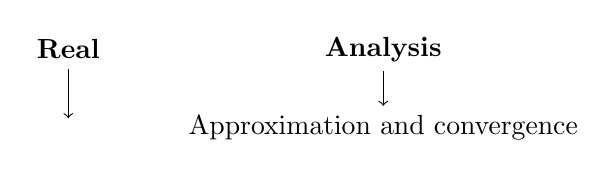
\begin{tikzpicture}
    \node (real) at (0,0) {\textbf{Real}};
    \node (analysis) at (4,0) {\textbf{Analysis}};
    \node (numbers) at (0,-1) {$\R$};
    \node (approximation) at (4,-1) {Approximation and convergence};
    \draw[->] (real) -- (numbers);
    \draw[->] (analysis) -- (approximation);
  \end{tikzpicture}
\end{center}

How do we rigorously define numbers? Numbers are defined by their properties.

\subsection{The Natural Numbers}

\begin{definition}{Natural Numbers}{natural-numbers}
  The set of \textbf{natural numbers} $\N$ has a \textbf{successor function}
  \[
    S\colon\N\to\N
  \]
  satisfying:
  \begin{enumerate}[label=(\arabic*)]
    \item There is an element $1\in\N$.
    \item For every $n\in\N$, $1\ne S(n)$.
    \item $S$ is injective.
    \item If $A\subseteq\N$ satisfies $1\in A$ and
          \[
            n\in A\implies S(n)\in A,
          \]
          then $A=\N$.
  \end{enumerate}
\end{definition}

\begin{itemize}
  \item For (1)--(3) in Definition~\ref{def:natural-numbers}, think of $S(n)=n+1$, although addition is not yet defined.
  \item Condition (4) rules out extra elements outside the successor chain starting at $1$, such as the separate cycle below.
\end{itemize}

\begin{center}
  \begin{tikzpicture}
    \node (one) at (0,0) {$1$};
    \node (two) at (1.5,0) {$2$};
    \node (three) at (3,0) {$3$};
    \node (dots) at (4.5,0) {$\cdots$};
    \draw[->] (one) -- node[above] {$S$} (two);
    \draw[->] (two) -- node[above] {$S$} (three);
    \draw[->] (three) -- node[above] {$S$} (dots);
    \node (alpha) at (6.5,0) {$\alpha$};
    \node (beta) at (8,0) {$\beta$};
    \draw[->] (alpha) to[bend left=45] node[above] {$S$} (beta);
    \draw[->] (beta) to[bend left=45] node[below] {$S$} (alpha);
  \end{tikzpicture}
\end{center}

\subsection{Addition}

\begin{definition}{Addition on the Natural Numbers}{natural-number-addition}
  Define addition recursively by
  \begin{align*}
    n+1    & := S(n),   &  & n\in\N,   \\
    n+S(m) & := S(n+m), &  & n,m\in\N.
  \end{align*}
\end{definition}

\begin{example}[Adding Using Successors]
  \begin{align*}
    2+3 & = 2+S(2)        \\
        & = S(2+2)        \\
        & = S(2+S(1))     \\
        & = S(S(2+1))     \\
        & = S(S(S(2)))    \\
        & = S(S(S(S(1)))) \\
        & = 5.
  \end{align*}
\end{example}

\subsection{Proof by Induction}

Axiom (4) in Definition~\ref{def:natural-numbers} is the basis for proof by induction.

\begin{theorem}{Principle of Mathematical Induction}{mathematical-induction}
  Suppose $P_1,P_2,\ldots,P_n,\ldots$ is a sequence of propositions such that
  \begin{enumerate}
    \item $P_1$ is true;
    \item $P_n\implies P_{n+1}$ for every $n\in\N$.
  \end{enumerate}
  Then $P_n$ is true for every $n\in\N$.
\end{theorem}

\begin{proof}
  Define $A=\{n\in\N : P_n\text{ is true}\}$.
  The hypotheses give $1\in A$ and $n\in A\implies S(n)=n+1\in A$.
  By axiom (4), $A=\N$.
\end{proof}
